\scanpage{9}\mspage{8}
J'explicite, à cause de son importance, la propriété suivante, bien qu'elle sera conséquence de diverses façons d'autres

\deleted{\uline{At} DC 1 : Soient $X,Y\in\unsure{M|\mathcal M}$ avec $X\deleted{\unsure{\parallel}}\mathrel{\tikz[baseline=-.4ex,x=.65em,y=.65em]{\draw (0,1.1)--(1,.5)--(0,-.1) (1,1.1)--(0,.5)--(1,-.1);}}Y\unsure{\text{\S}|?|.}$}
\deleted{\deleted{\unsure{Alors}} \inserted{Soient} $X'\ll X$, \deleted{$Y'\ll Y\Longrightarrow X'\parallel Y'$} \inserted{avec $X'\parallel X\cap Y=L$, (i.e. $X'\parallel Z$ pour $Z\leq X,Y$)} $Y'\ll Y$ avec $Y'\parallel L$. Alors $X'\parallel Y'$}

% slanted
\margin{\uline{NB} La chose importante est $X'\mathrel{\tikz[baseline=-.4ex,x=.65em,y=.65em]{\draw (0,1.1)--(1,.5)--(0,-.1) (1,1.1)--(0,.5)--(1,-.1);}}Y'$, alors $X'\cap Y'=\unsure{\varphi|\varnothing}$ immédiat. Car $Z\deleted{\ll}\leq X',\,Z\leq Y'$ $\Longrightarrow Z\ll\unsure{X'|X},\,\unsure{Z'|Z}\ll\unsure{Y'|Y}$ d'où $Z\ll X\cap Y=L$, or $Z\leq X'\parallel L\Longrightarrow Z\parallel L$, or $Z\ll L$ et $Z\parallel L$ \deleted{\unsure{impossible}} (\unsure{comme|d'où} $Z\mathrel{\tikz[baseline=-.4ex,x=.65em,y=.65em]{\draw (0,1.1)--(1,.5)--(0,-.1) (1,1.1)--(0,.5)--(1,-.1);}}L$) $\Longrightarrow\unsure{Z^{+}\leq L|Z+\leq L|Z\leq L}$ \deleted{\unsure{absurde}} car \uline{$Z\cap L=\varphi$ !}}%

\deleted{\uline{Cor} 1 Soient $F,C\in\unsure{\mathscr F|\mathcal F}$ avec $F\parallel C$. Alors $F\ll F$, $C'\ll G\Longrightarrow F'\parallel G'$.}
\deleted{\uline{Cor. 2} Soient $F,G\in\mathscr F$, $F\mathrel{\tikz[baseline=-.4ex,x=.65em,y=.65em]{\draw (0,1.1)--(1,.5)--(0,-.1) (1,1.1)--(0,.5)--(1,-.1);}}G$ \deleted{$\unsure{L=\underset{Z\in\widetilde F\cap\widetilde G}{\mathrm{Sup}}\,Z}$} \inserted{$L=F\cap G$}, $F'\ll F,C'\ll G$. Supposons $F'\parallel L,\ C'\parallel L$, alors $F'\parallel G'$.}

\deleted{\uline{At DC} 2 \quad (Axiome des ateliers \unsure{spacieux|spécieux}) \deleted{\unsure{Soit|Soient}} $X,Y\in M$, $\deleted{\unsure{L}}K=X\cap Y=\underset{Z\in\widetilde X\cap\widetilde Y}{\mathrm{Sup}}\,Z$. Supposons que pour tt $X',Y'$, avec $X'\ll X,\underset{\tikz[x=1em,y=.35em,baseline=0pt]{\draw (0,0) .. controls (1,-.05) and (2,-.05) .. (3.4,.40);\draw (1.66,.16)--(1.85,.01)--(1.67,-.13);}}{Y'\ll Y,\ X'\parallel K},Y'\parallel K$, on ait $X'\parallel Y'$. Alors}

% Editing stroke beneath the preceding cancelled draft, with rising right end.
\noindent\tikz[x=1em,y=1em]{\draw (0,.03) .. controls (2,.15) and (4,.18) .. (6,.12) .. controls (8,-.04) and (10,-.10) .. (11.1,-.08) .. controls (11.45,.55) and (11.55,.95) .. (12.2,1.18);}

On voudra la

\uline{Propriété 1} Soient $F,G\in\mathscr F$, $F\mathrel{\tikz[baseline=-.4ex,x=.65em,y=.65em]{\draw (0,1.1)--(1,.5)--(0,-.1) (1,1.1)--(0,.5)--(1,-.1);}}G$, $L=F\cap G$. Soient $F'\ll F,\ G'\ll G$. Alors
\[
\begin{aligned}
 & F'\mathrel{\tikz[baseline=-.4ex,x=.65em,y=.65em]{\draw (0,1.1)--(1,.5)--(0,-.1) (1,1.1)--(0,.5)--(1,-.1);}}G'\\
\Longleftrightarrow\quad & F'_{L}\mathrel{\tikz[baseline=-.4ex,x=.65em,y=.65em]{\draw (0,1.1)--(1,.5)--(0,-.1) (1,1.1)--(0,.5)--(1,-.1);}}G'_{L}
\end{aligned}
\]

cf \deleted{\unsure{p.}} GF $\underline{\overline{\mathrm{VI}}}$, p.~\uline{\unsure{73|13}} -- On a en tous cas tjrs $\unsure{\mathrel{\tikz[x=.5em,y=.28em]{\draw (0,.08)--(1.2,.08) (0,.42)--(1.2,.42) .. controls (1.35,.42) and (1.38,.23) .. (1.28,.2);}}|\Rightarrow}$
\deleted{\unsure{Montrons} qu'on a bien \unsure{en} $\Rightarrow$. En effet,}

Ceci est équivalent (si on le voit de façon générale) à l'ancien At 12, qui prend le nom

% slanted
\margin{\uline{Critère} de \uline{compatibilité} pour les raffinements de \uline{sous-figures}\quad Mais c'est faux dans le cas simplicial, ex :}%
\figure{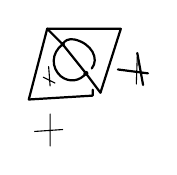
\begin{tikzpicture}[x=.035em,y=-.035em,line cap=round,line join=round]
\draw[thick] (30,10)--(106,10)--(85,76);
\draw[thick] (30,10)--(11,83)--(77,79)--(77,73);
\draw[thick] (30,10)--(46,26)--(70,56)--(85,76);
\draw[thick] (76,51) .. controls (84,41) and (76,25) .. (58,21)
 .. controls (52,20) and (48,22) .. (46,26)
 .. controls (34,35) and (34,50) .. (44,59)
 .. controls (53,66) and (64,64) .. (70,56);
\fill (46,26) circle (2.2) (70,56) circle (2.6);
\draw (26,60)--(38,66) (31.5,49)--(33,69);
\draw[thick] (103,52)--(134,56) (123,35)--(129,68);
\draw (123,39)--(122,67);
\draw (17,116)--(46,114) (33,98)--(33,131);
\end{tikzpicture}}
% slanted
\margin{Mais on aura $X'_{L}\parallel Y'_{L}\Longrightarrow X'\mathrel{\tikz[x=.55em,y=.60em,line cap=round]{\draw (0,-.12)--(0,1) (.48,-.12)--(.48,1) (-.06,.30)--(.54,.47) (-.05,.51)--(.53,.65);}}Y'$, C'est un contre-exple à l' : At $\parallel$, et a fortiori à \deleted{\unsure{ex}} At 11 (cf GF $\underline{\overline{\mathrm{VI}}}$, p. 67,68)}%

% Vertical rule bordering the axiom on its left.
\margin{\tikz[x=.5em,y=.5em]{\draw (0,0)--(0,4.25);}}
\uline{At \unsure{DD|CD|DC}} 1 Soient \inserted{ou bien} $X,Y\ \unsure{o|et|,}\ X',Y'\in M$, $X\mathrel{\tikz[baseline=-.4ex,x=.65em,y=.65em]{\draw (0,1.1)--(1,.5)--(0,-.1) (1,1.1)--(0,.5)--(1,-.1);}}Y,\ X'\ll X,Y'\ll Y$. Posons $K=X\cap Y=\underset{Z\in\widetilde X\cap\widetilde Y}{\mathrm{Sup}}\,Z$. Alors $X'_{L}\mathrel{\tikz[baseline=-.4ex,x=.65em,y=.65em]{\draw (0,1.1)--(1,.5)--(0,-.1) (1,1.1)--(0,.5)--(1,-.1);}}Y'_{L}$ implique $X'\mathrel{\tikz[baseline=-.4ex,x=.65em,y=.65em]{\draw (0,1.1)--(1,.5)--(0,-.1) (1,1.1)--(0,.5)--(1,-.1);}}Y'$ \quad (NB l'inverse \deleted{\unsure{est}} tjrs vrai)

\uline{Cor. Main} 1 \quad la ``propriété'' ci dessus

\[
F\parallel G,\ F'\ll F,\ C'\ll G\ \Longrightarrow\ F'\parallel G'
\tag*{\makebox[0pt][r]{\makebox[\displaywidth][l]{\uline{Cor. Main} 2}}}
\]

Plus gén. \quad Si $F\mathrel{\tikz[baseline=-.4ex,x=.65em,y=.65em]{\draw (0,1.1)--(1,.5)--(0,-.1) (1,1.1)--(0,.5)--(1,-.1);}}G,\ F'\ll F,\ C'\ll G$, alors
\[
 F'\parallel G'\ \Longleftrightarrow\ F'_{L}\parallel G'_{L}
\]
